%{
% \documentclass[12pt,ngerman]{/Users/dominik-cau/Documents/Lernen/Uni/Promotion/Vorlagen/Bayreuth/Exercise/AssignmentClass}
\documentclass[12pt,ngerman]{AssignmentClass}
% \documentclass{article}
%\documentclass[12pt, english]{AssignmentClass}


%----------------------------------------------------------------------------------------
%	PACKAGES AND OTHER DOCUMENT CONFIGURATIONS
%----------------------------------------------------------------------------------------
% Template-specific packages
\usepackage[utf8]{inputenc} % Required for inputting international characters
\usepackage[T1]{fontenc} % Output font encoding for international characters
\usepackage{mathpazo} % Use the Palatino font
\usepackage{wasysym} % for flash-symbol
\usepackage{graphicx} % Required for including images
\usepackage{amsmath}
\usepackage{listings} % Required for insertion of code
\usepackage{siunitx}
\usepackage{pnets}
\usepackage[most]{tcolorbox} % Grey Deadline Bar
\DeclareMathAlphabet{\mathpzc}{OT1}{pzc}{m}{it}
% Initialize comment sections
\usetheme{light-theme}
\excludecomment{dark-theme}
\excludecomment{solution}


%----------------------------------------------------------------------------------------
%	SET VERSION
%----------------------------------------------------------------------------------------
%\includecomment{dark-theme}
\includecomment{solution}


%----------------------------------------------------------------------------------------
%	ASSIGNMENT INFORMATION
%----------------------------------------------------------------------------------------
%\setlanguageEnglish
%\setlanguageGerman
% \begin{dark-theme}
% 	\usetheme{dark-theme}
% 	\excludecomment{light-theme}
% \end{dark-theme}
\title{Übung 1 Lösung} % Assignment title
\instructor{Yorck Zisgen}
\class{Generative Künstliche Intelligenz} % Course or class name
\term{Sommersemester 2024}
% \topics{Begriffe $\bullet$ Kontrollflussmuster $\bullet$ Organisationseinheiten}
\topics{07.05.2024}
%----------------------------------------------------------------------------------------
%}

\begin{document}
	\maketitle

    % Header Deadline Bar
    %{
    \noindent % Ensures the box spans the entire width
    \begin{tcolorbox}[colback=gray!20, % Background color as light gray
                      colframe=gray!20, % Frame color same as background
                      boxrule=0pt, % No border
                      sharp corners, % Sharp corners
                      valign=center, % Vertically centered text
                      halign=center, % Horizontally centered text
                      height=2cm] % Height of the box
    \LARGE \bfseries Beispiellösung % Bold text
    \end{tcolorbox}
    %}

    
    \section{Modellierung vs. Machine Learning}
        Erklären Sie den Unterschied zwischen klassischer Modellierung und Machine Learning Ansätzen. Geben Sie jeweils ein Beispiel.

        \vspace{5mm}
        Die Lösung hierzu findet sich in Foliensatz 1 auf Folie 27. In der klassischen Modellierung wird ein Modell angefertigt. Anschließend werden erhobene Daten in das Modell gegeben. Das Modell berechnet auf Basis dieser Daten ein Ergebnis.
        Supervised Machine Learning Ansätze geben gelabelte Trainingsdaten in einen Algorhithmus. Hieraus entsteht als 'Black Box' ein trainiertes Modell. Dieses Modell ist nun in der Lage, auch ungelabelte Daten auf Basis des Trainings zu verarbeiten.
        Ausgangspunkt der Modellierung ist also das Modell, beim Supervised Machine Learning ist der Ausgangspunkt die Trainingsdatenmenge.
        Beispiele für die klassische Modellierung wären Simulationen oder Geschäftsprognosen. Ein Beispiel für Machine Learning wäre Optical Recognition.       


    
    
    \section{Grenzen von LLMs}
        
        \begin{enumerate}[a)]
            \item Diskutieren Sie die aktuellen Grenzen von LLMs. Welche Möglichkeiten sehen Sie, diese zu beheben?
            \item Testen Sie folgendes mit ChatGPT: Wörter invertieren, Galgenraten, 4 Gewinnt, TicTacToe spielen. Fassen Sie kurz die Ergebnisse Ihrer Evaluation zusammen.
        \end{enumerate}

        \vspace{5mm}
        Die Grenzen von LLMs werden in Foliensatz 1 auf Folie 18 dargestellt:
        \begin{itemize}
            \item Rechenleistung -> vermutlich technisch keine Verbesserung möglich
            \item Datenqualität -> Bessere Auswahl von Trainingsdaten
            \item Datenbestand -> Aktualisierung des Datenbestands, Erweiterung zu Echtzeit-Lernen
            \item Halluzination -> stets hinterfragen.
            \item Bias -> Aufmerksamkeit bei der Auswahl der Trainingsdaten
            \item Datenschutz und Datensicherheit -> Lokale LLMs, Training auf Eingabe verbieten
            \item Fehlende Quellenangaben -> manuelle Recherche
            \item Fehlende Zitierwürdigkeit -> im wissenschaftlichen Umfeld nicht vollständig lösbar. Berücksichtigung der Vorgaben des Prüfungsamtes/Studiendekanats, verwenden von spezialisierten LLMs wie consensus.app
        \end{itemize}

        \begin{itemize}
            \item Wörter invertieren gelingt überwiegend, aber nicht durchgängig. Lagerregal und Lollipop bereiteten ChatGPT Probleme.
        \end{itemize}
        
        \begin{figure}
            \centering
            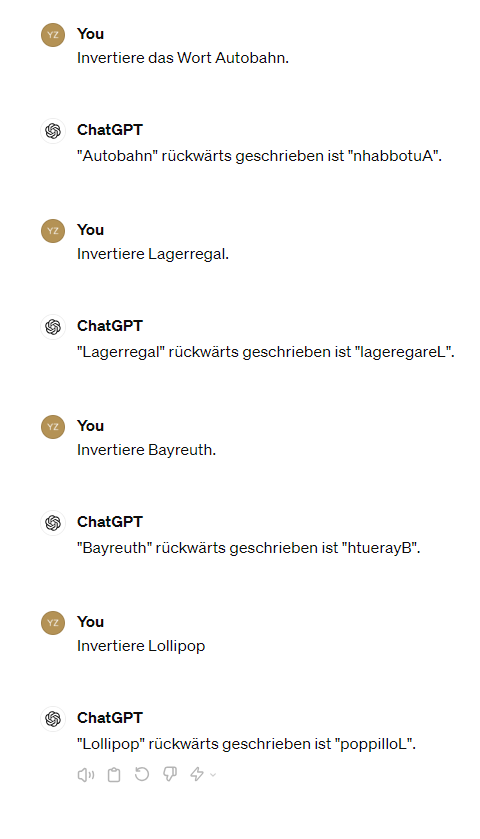
\includegraphics[width=0.5\linewidth]{2024-04-22 09_50_43-ChatGPT.png}
            \caption{Wörter invertieren}
            \label{fig:inverted_words}
        \end{figure}

        \begin{itemize}
            \item Galgenraten ist nicht sinnvoll spielbar.
        \end{itemize}
        
        \begin{figure}
            \centering
            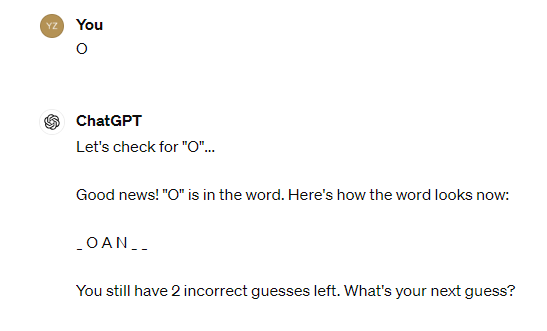
\includegraphics[width=0.5\linewidth]{2024-04-22 09_44_49-Play TicTacToe with Me.png}
            \caption{Galgenraten 1}
            \label{fig:hangman_1}
        \end{figure}
        \begin{figure}
            \centering
            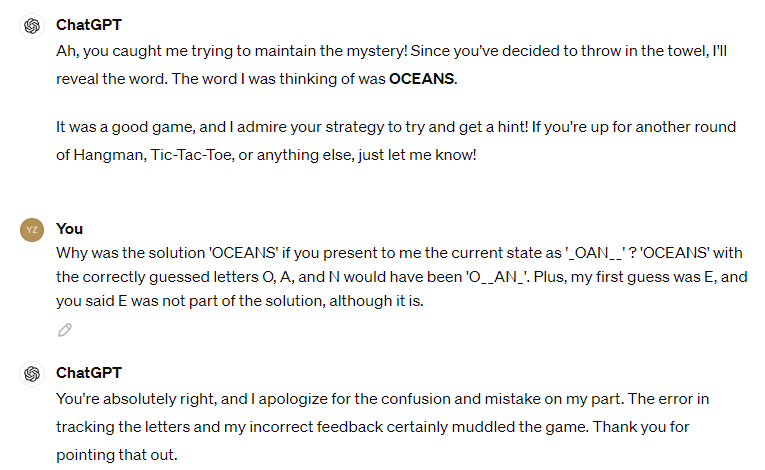
\includegraphics[width=0.5\linewidth]{2024-04-22 09_45_28-Play TicTacToe with Me.png}
            \caption{Galgenraten 2}
            \label{fig:hangman_2}
        \end{figure}

        \begin{itemize}
            \item TicTacToe und 4 Gewinnt sind beides Spiele, bei denen ChatGPT mit einem 'Spielfeld' umgehen können muss. Hierbei kommt es immer wieder zum Phänomen, dass Spielfelder ihren Wert wechseln oder Zusammenhänge (4 in einer Reihe) nicht als solche erkannt werden. ChatGPT repräsentiert Wörter intern als eine Reihe von Tokens statt einer Reihe von Buchstaben. Hierdurch kommt es zu Problemen bei Aufgaben auf Buchstabenebene.
        \end{itemize}
    
    
    \section{Praktische Anwendung}
    
        \begin{enumerate}[a)]
    		\item Lassen Sie von ChatGPT eine Modulbeschreibung zu einer Vorlesung schreiben, die „Einführung in die Generative KI“ heißt. Die Vorlesung ist für Masterstudierende der Wirtschaftswissenschaften gedacht.
    		\item Lassen Sie sich eine Übungsaufgabe zu der Vorlesung erstellen.
    		\item Erstellen Sie 5 Quizaufgaben zu der Vorlesung.
            \item Suchen Sie nach einem Beispiel, bei dem ChatGPT halluziniert.
    	\end{enumerate}

        \vspace{5mm}
        Beispielhafte Prompts:
        \begin{enumerate}[a)]
    		\item 'Erstelle eine Modulbeschreibung für die Mastervorlesung 'Einführung in die Generative KI'. Zielgruppe sind Studierende der Wirtschaftswissenschaften.'
    		\item 'Erstelle eine Übungsaufgabe zu dieser Vorlesung. Die Bearbeitung der Aufgabe sollte einen Umfang von ca. 10 Minuten haben.'
    		\item 'Erstelle 5 Quizfragen zu der Vorlesung.'
            \item 'Nenne mir 5 Mitglieder der aktuellen Bundesregierung.'
    	\end{enumerate}

        \begin{figure}
            \centering
            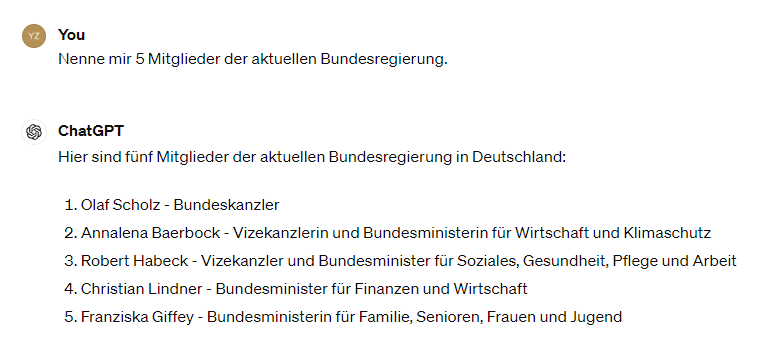
\includegraphics[width=0.5\linewidth]{2024-04-22 10_18_58-ChatGPT.png}
            \caption{Halluzinationen}
            \label{fig:hallucinations}
        \end{figure}
    
    
    \section{Kombinierte Anwendung}
    
        Generative KI kann nicht nur Texte erstellen.
        
        \begin{enumerate}[a)]
            \item Wählen sie ein Aufgabengebiet (Text-to-X oder X-to-Text). Recherchieren sie hierzu drei mögliche Produkte. Ermitteln Sie, ob sich manche davon kostenlos nutzen lassen.
            \item Denken Sie sich ein Produkt aus und erzeugen Sie zu diesem Produkt eine Produktbeschreibung und ein fiktives Bild.
            \item Erzeugen sie eine Homepage, auf der Produktname, -Bild und -Beschreibung dargestellt werden. [\textit{Hinweis: ChatGPT-3.5 kann keine Bilder erzeugen. Sie können ChatGPT-4.0 verwenden wenn Sie Zugriff darauf haben, eine Alternative wie bspw. https://deepai.org benutzen oder etwas anderes wie einen Werbetext oder ein Video erzeugen.}]
        \end{enumerate}
        

        \vspace{5mm}
        \noindent Beispielprompt zu Teilaufgaben b) und c) :\\
        \textit{I have invented a new product, called 'Stygian Strider'. It is a comfortable Sneaker. Create a product description. Then create an image based on your description. Then create a HTML code that displays name, image, and description. Let's do this step-by-step.}

        \begin{figure}
            \centering
            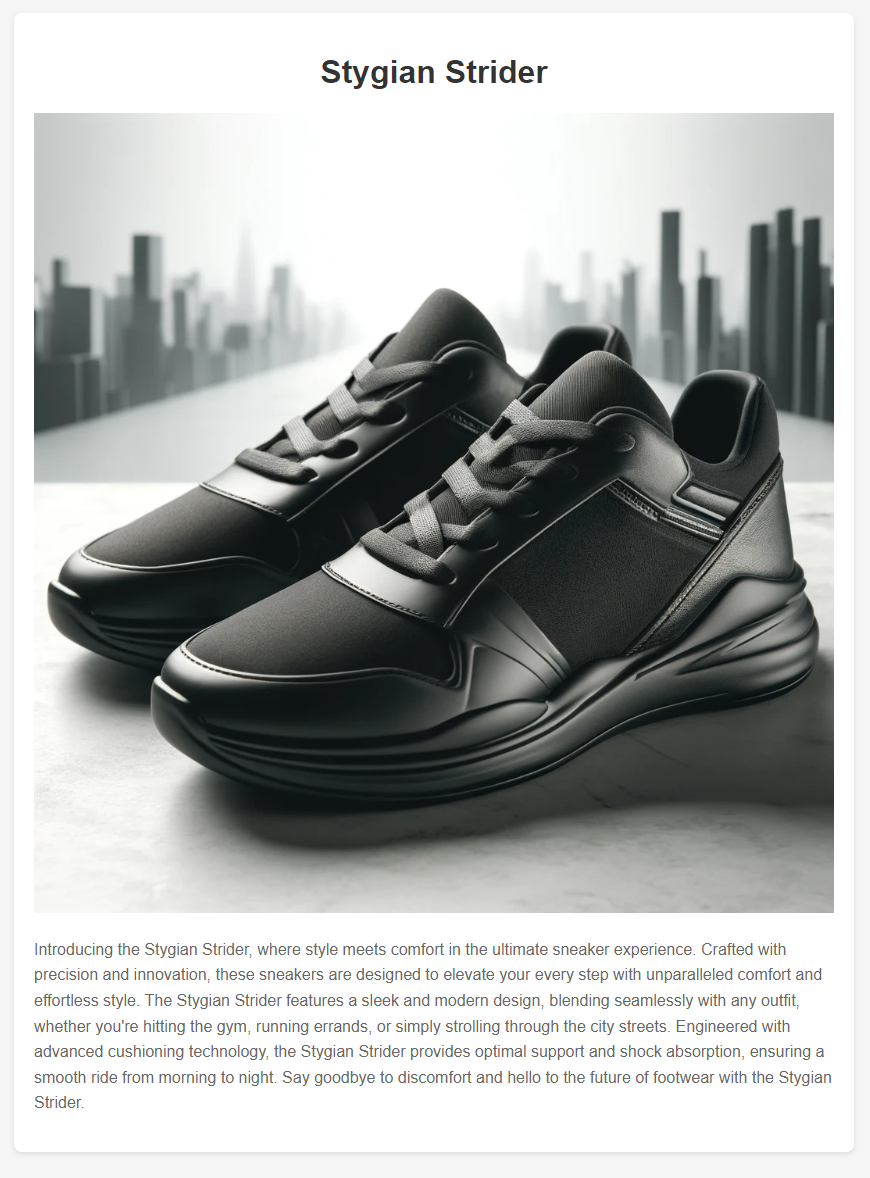
\includegraphics[width=0.5\linewidth]{2024-04-22 10_37_14-Stygian Strider.png}
            \caption{Produktname, -bild und -homepage (DALL-E/ChatGPT-4.0)}
            \label{fig:product}
        \end{figure}
    
\end{document}

